\chapter{A proof of concept method to identify enhancers using grammatical constraints on binding site motifs}

%%%%%%%%%%%%%%%%%%%%%%%%%%%%%%%%%%%%%%%%%%%%%%%%%%%%%%%%%%%%%%%%%%%%%%%%%%%%%%%%
\section{Introduction}
%%%%%%%%%%%%%%%%%%%%%%%%%%%%%%%%%%%%%%%%%%%%%%%%%%%%%%%%%%%%%%%%%%%%%%%%%%%%%%%%

Enhancers are non-coding elements of the human genome that act as switches to regulate when and where genes are expressed. This feature of enhancers thus makes them a key contributor to tissue-specific gene expression during tightly controlled processes such as development and homeostasis [CITE]. Most disease mutations are located within enhancers [CITE]. However, there is still a lack of understanding of how genomic sequence relates to proper or improper enhancer function [CITE]. With the increasing volume of genomic data collected due to next-generation sequencing [CITE], it is necessary to develop computational tools to mine genomes to pinpoint tissue-specific enhancers for further study. 

Computational tools to identify enhancers have primarily focused on chromatin signatures [CITE]. While tissue-specific epigenomic data can sometimes pinpoint tissue-specific enhancers [CITE], this approach largely ignores the possible link between transcription factor binding site (TFBS) organization, or enhancer grammar, and tissue-specific activity [CITE]. Currently, three different models for enhancer-TFBS interactions have been proposed. The billboard model suggests that there are no constraints on TFBS arrangements within an enhancer—only that TFBSs be present somewhere in the sequence [CITE]. In contrast, the enhanceosome model suggests that TFBSs must reside in a precise arrangement within an enhancer [CITE]. Finally, the TF-collective model suggests that in the absence of TFBS organization within an enhancer sequence, there is collective occupancy of the enhancer sequence by transcription factors (TF) through a combination of direct TF binding to TFBSs and TF-TF interactions [CITE]. While we have found representative examples for each enhancer-TFBS interaction model, we still lack the computational tools to annotate grammatically interesting genomic regions. 

In a previous study, we found that there may be grammatical rules governing notochord enhancers regulated by three different groupings of Zic, ETS, Brachyury (Bra), and FoxA TFBSs: (1) Zic and ETS; (2) Zic, ETS, and Bra; and (3) Zic, ETS, Bra, and FoxA [CITE]. Interestingly, when testing genomic regions from the organism \textit{Ciona intestinalis type A} (\textit{Ciona}) containing these sites, we came to the striking conclusion that clusters of binding sites alone are not sufficient to drive expression even though all the transcription factors at play have some biological association with the nervous system or notochord [CITE]. Here, we focus on expanding the scope of the previous study to understand how enhancers regulated by Zic and ETS encode notochord expression within \textit{Ciona} using an updated genomic reference sequence developed after we performed our initial screen [CITE]. We have also developed EnGAGE (Entire Genome seArches for Grammars of Enhancers), a computational framework to search for tissue-specific enhancers within genomes using knowledge of enhancer grammar or motif signatures. In the following, we demonstrate the synergy between EnGAGE and massively parallel reporter assays (MPRAs) to study the \textit{Ciona} notochord enhancer grammar consisting of Zic, ETS, Bra, and FoxA TFBSs [CITE]. 

%%%%%%%%%%%%%%%%%%%%%%%%%%%%%%%%%%%%%%%%%%%%%%%%%%%%%%%%%%%%%%%%%%%%%%%%%%%%%%%%
\section{Results}
%%%%%%%%%%%%%%%%%%%%%%%%%%%%%%%%%%%%%%%%%%%%%%%%%%%%%%%%%%%%%%%%%%%%%%%%%%%%%%%%

\subsection{Searching for clusters of Zic and ETS sites within an updated \textit{Ciona} genome}

In our previous study, we identified regions across the \textit{Ciona} genome containing one Zic site and at least two ETS sites within 30 bp of the Zic site [CITE]. While we were able to identify a suitable number of ZEE elements to perform an enhancer screen, there were two key limitations in our initial search methodology that we wanted to address in an updated search. The first limitation was the genomic reference used for \textit{Ciona}. While completing the analyses for our previous study, a new genomic reference for \textit{Ciona} was released using more modern next-generation sequencing methods—the previous genome reference was assembled in 2008 [CITE]. The second limitation of our previous search was the inherent search design itself. Because we fixed the Zic site in the center of the genomic element, we potentially missed functional ZEE elements that did not follow this constraint. To continue studying the notochord dependency grammar we previously identified at a greater scale, we developed a new search methodology that improved upon these limitations [CITE]. We improved our methods by first using the updated \textit{Ciona} genomic reference and allowing for more flexibility in binding site location when searching for regions of interest containing Zic and ETS. 

For the next iteration of our search, we identified 100 bp regions in the updated \textit{Ciona} genome containing at least one Zic site and at least two non-overlapping ETS sites. Like our previous approach, we searched for ETS sites using the core motif, \verb|GGAW| (\verb|GGAA| or \verb|GGAT|), to consider all ETS sites regardless of affinity [CITE]. We also defined Zic sites using EMSA and enhancer mutagenesis data from previous studies [CITE]. Using this approach, we identified 4,434 regions with at least one Zic and two ETS sites [TABLE]. Within this study, we define these regions as KYN elements to reference the new “KY” \textit{Ciona} genome assembly, and we are looking at “N,” or notochord, grammars. In our previous study, we found at least three groups of factors governed those notochord enhancers: (1) Zic and ETS, (2) Zic, ETS, and Brachyury (Bra), and (3) Zic, ETS, Bra, and FoxA [CITE]. In associating our KYN elements with each of these groups [FIGURE], we found that 65\% belonged to the Zic/ETS group (2,863 KYN elements), 31\% belonged to the Zic/ETS/FoxA group (1,384 KYN elements), and 4\% belonged to the Zic/ETS/FoxA/Bra group (187 KYN elements). 

After determining our genomic elements of interest, we wanted to evaluate how many ZEE elements exist within the new KYN library using Magic-BLAST [CITE]. We created a custom BLAST database using the KYN elements as a reference, then searched for our ZEE elements within this custom database. Of the ZEE elements included in our previous study, 77\% were present (69/90) in our new KYN elements (Figure \ref{fig:1 zee comparison}). Additionally, 78\% of the ZEE elements expressed in the notochord were present in the KYN library, including the Brachyury Shadow (BraS) enhancer and the LAMA1/3/5 and LRIG1/2/3 enhancers, which our studies have previously identified (Figure \ref{fig:1 zee comparison}). Additionally, one element, ZEE86, matched two KYN elements—KYN2713 and KYN4077 (Figure \ref{fig:1 zee comparison}). 

\begin{landscape}
    \begin{figure}[h]
        \centering
        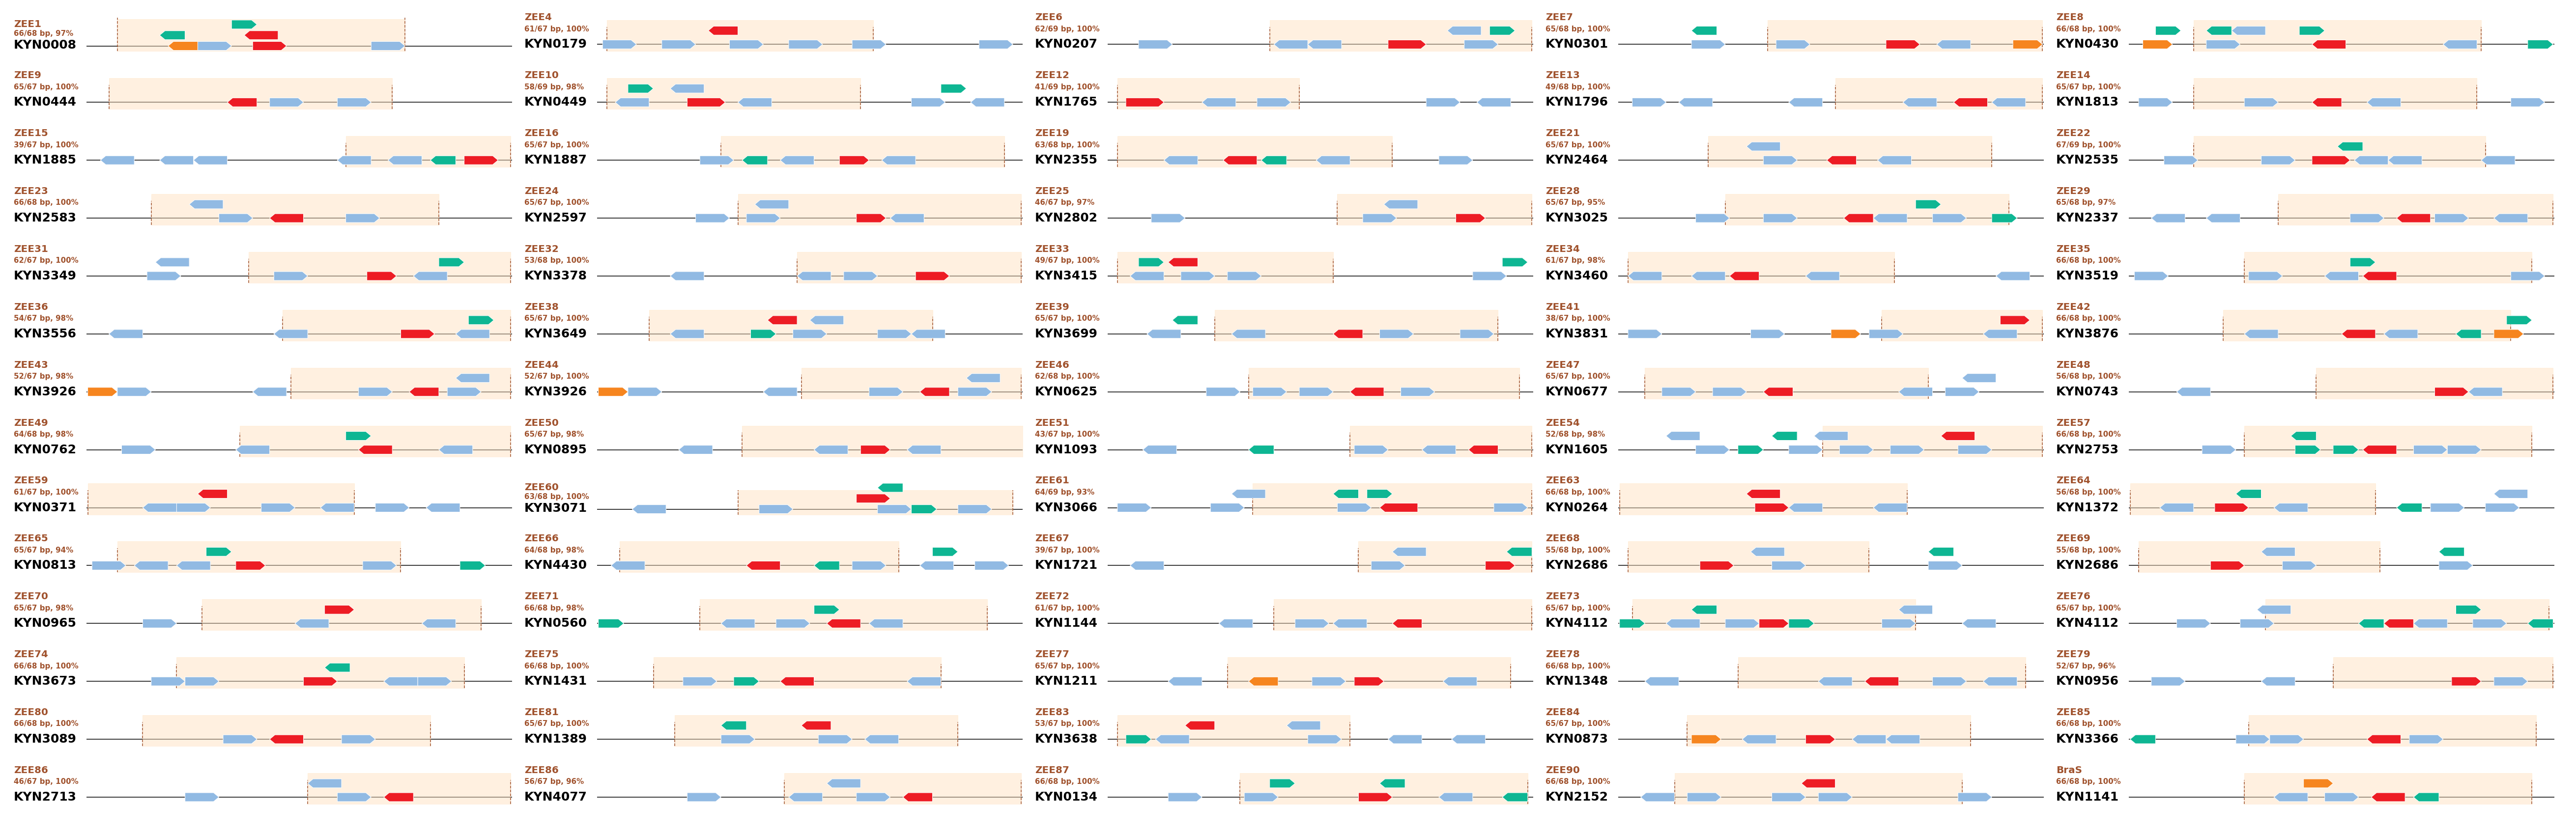
\includegraphics[scale=0.12]{3_figures-and-files/Fig1_ZEE-Comparison.png}
        \caption[The majority of ZEE sequences can be found in the KYN library]{\textbf{The majority of ZEE sequences can be found in the KYN library.} 
        As determined by Magic-BLAST, a total of 69/90 ZEE elements were found to overlap with members of the KYN library. Each diagram represented in the figure represents a schematic of the KYN enhancer, where the highlighted region represents the overlapping ZEE element that was detected by Magic-BLAST. The number of bases that aligned, along with the percentage alignment is also indicated. The colored binding sites represent the order, orientation, and spacing of Zic (red), ETS (blue), Bra (green), and FoxA (orange).}
        \label{fig:1 zee comparison}
    \end{figure}
\end{landscape}

\subsection{Evaluating KYN genomic elements for enhancer activity in developing \textit{Ciona} embryos}

Next, we wanted to determine which KYN elements were functional by conducting an enhancer screen. We synthesized all 4,434 KYN elements upstream of a minimal promoter (bpFog) and a transcribable barcode. In addition to the ZEE elements that drove notochord expression in the previous study [CITE], we wanted to evaluate how centering the Zic site within the sequence would impact expression. Thus, we took the sequences for the ZEE element with the highest enhancer activity, ZEE1 or LRIG1/2/3, and BraS, and centered the Zic site based on the sequence present in the updated \textit{Ciona} genome. Finally, we wanted to test the necessity of Zic and ETS for a given KYN element. To do this, we ablated the core of the Zic (\verb|GCWG| to \verb|GAWG|) and the core of the ETS (\verb|GGAW| to \verb|GCAW|) binding sites for each of the KYN elements and then included these sequences within the library. 

Our enhancer screen included 8,872 sequences, each associated with, on average, 88 barcodes. Each barcode represents a specific measurement of enhancer activity. We then electroporated the enhancer library into fertilized \textit{Ciona} eggs. We collected embryos at the late gastrula stage (5.5 hours post fertilization, hpf), as this stage is where notochord cells are developing, and both Zic and ETS are expressed [CITE]. At this time point, we isolated both the mRNA and plasmid DNA and then sequenced the mRNA and DNA barcodes present. We filtered the data based on if a barcode was present for an enhancer and if the Zic/ETS-ablated form of the enhancer was present within the data. In total, our library had 81\% of our expected sequences present (7,226/8,872 KYN sequences), including 86\% of the sequences that overlapped with the ZEE library (60/70 ZEE elements with successful KYN hits).

Next, we determined which KYN elements act as enhancers by calculating an activity score for each element. We first calculated the reads per million (RPM) for each mRNA and DNA barcode, then averaged the RPM across the mRNA and DNA barcodes associated with a given KYN element. To normalize the enhancer activity to differences in the amount of plasmid electroporated into each embryo, we took the log2 of the average enhancer activity—mRNA RPM—divided by the average plasmid present—DNA RPM—for the same enhancer. The lowest and highest activity score detected were 1.02 and 4.99, respectively.

Several active KYN enhancers are proximal to genes implicated in the notochord and nervous system
In our enhancer screen, we were interested in identifying enhancers that would decrease in expression upon ablation of the Zic and ETS binding sites to ensure the importance of these sites in conferring activity in our \textit{Ciona} embryos. We first filtered for functional enhancers by filtering for non-ablated regions with an activity score greater than or equal to the 90th percentile of the mean activity score or an activity score of 2.26. Next, we divided this group into three subsets based on their present grammar pattern: Zic/ETS, Zic/ETS/Bra, or Zic/ETS/Bra/FoxA. For the enhancers in each of these three groups, we then kept them within our subset of active enhancers if their ablated sequence was present below the 90th percentile cutoff. In total, we identified 438 active Zic/ETS regions, 204 active Zic/ETS/Bra regions, and 29 Zic/ETS/Bra/FoxA regions. 

To identify the top candidates from each category to evaluate further, we calculated the difference in enhancer activity between the “normal” and “ablated” sequences and sorted enhancers by this value. We then determined proximal genes by expanding approximately 5 kb on either edge of the sequence and annotating genes within this expanded window as proximal to our region of interest. The top five candidates within each category can be found in Table \ref{tab:top kyn elements across grammars}.

Upon looking over the top candidates, we see the largest differences between normal and their ablated variants in the Zic/ETS and Zic/ETS/Bra grammatical categories, whereas we see almost minimal difference between the normal and ablated variants in the Zic/ETS/Bra/FoxA category. When reviewing the top five candidates from each grammatical category, we were surprised to find multiple genes implicated in nervous system disorders, especially regarding brain-associated conditions, such as \textit{RGS8}, \textit{RGS4}, \textit{SYS1}, \textit{ALDH4A1}, \textit{WARS2}, \textit{ITPR1}, \textit{XRN2}, \textit{KCNQ3}, and \textit{OTX1}. Several genes were also implicated in skeletal and bone-related disorders, such as \textit{HOXD3}, \textit{DYNLT2B}, and \textit{FLG}. Ultimately, more exploration is needed to discern if these regions are truly functional within \textit{Ciona} through imaging studies, but their primary association with homologous human genes is promising. 

\begin{small}
    \begin{landscape} % this table is long, so it'll be multi-page landscape
        \begin{longtable}{l l p{.18\textwidth} p{.15\textwidth} p{.15\textwidth} p{.15\textwidth} p{.2\textwidth}}
            % Define the table title in the table of contents
            \caption{Top KYN elements across grammatical categories} 
            \label{tab:top kyn elements across grammars}
            \\ \hline 

            % Define the table columns for the first and all subsequent pages
            \multicolumn{1}{l}{\textbf{GRAMMAR}} & \multicolumn{1}{l}{\textbf{KYN ID}} & \multicolumn{1}{l}{\textbf{LOCATION}} & \multicolumn{1}{l}{\textbf{ACTIVITY(N)}} & \multicolumn{1}{l}{\textbf{ACTIVITY(A)}} & \multicolumn{1}{l}{\textbf{ACTIVITY(N-A)}} & \multicolumn{1}{l}{\textbf{PROXIMAL GENES}} \\ \hline \endfirsthead

            \multicolumn{7}{l}%
            {{\textbf{\tablename\ \thetable{}.} Top KYN elements across grammatical categories, \textit{continued from previous page}}} \\
            \hline 
            \multicolumn{1}{l}{\textbf{GRAMMAR}} & \multicolumn{1}{l}{\textbf{KYN ID}} & \multicolumn{1}{l}{\textbf{LOCATION}} & \multicolumn{1}{l}{\textbf{ACTIVITY(N)}} & \multicolumn{1}{l}{\textbf{ACTIVITY(A)}} & \multicolumn{1}{l}{\textbf{ACTIVITY(N-A)}} & \multicolumn{1}{l}{\textbf{PROXIMAL GENES}} \\
            \hline\hline \endhead

            % Define the table footer for the first and all subsequent pages
            \hline \multicolumn{7}{r}{\textit{Continued on next page}} \\ \hline \endfoot
            \hline \endlastfoot
            
            % Start table content

            %%%%% %%%%% %%%%% %%%%% %%%%% %%%%% %%%%% %%%%% %%%%% %%%%% %%%%% %%%%%
            Zic/ETS & KYN4389 & chr9:2616602-2616702 & 4.57 & 1.98 & 2.59 & \textit{POM121L2}, \textit{RGS8}, \textit{RGS4} \\
            Zic/ETS & KYN4390 & chr9:2616623-2616723 & 4.26 & 1.97 & 2.29 & \textit{POM121L2}, \textit{RGS8}, \textit{RGS4} \\
            Zic/ETS & KYN1765 & chr2:2253506-2253606 & 3.38 & 1.58 & 1.79 & \textit{ERCC5}, \textit{SYS1}, \textit{ESD} \\
            Zic/ETS & KYN0616 & chr10:1184720-1184820 & 3.75 & 1.99 & 1.76 & \textit{ALDH4A1}, \textit{CBL} \\
            Zic/ETS & KYN0516 & chr1:14250867-14250967 & 3.61 & 1.95 & 1.66 & \textit{HOXD3}, \textit{DYNLT2B} \\
            
            Zic/ETS/Bra & KYN2946 & chr6:381260-381360 & 4.79 & 1.71 & 3.08 & \textit{WARS2} \\
            Zic/ETS/Bra & KYN3554 & chr8:5563238-5563338 & 2.79 & 1.33 & 1.46 & \textit{ITPR1} \\
            Zic/ETS/Bra & KYN0942 & chr11:2883954-2884054 & 2.74 & 1.37 & 1.36 & \textit{YME1L1} \\
            Zic/ETS/Bra & KYN2661 & chr4:6611261-6611361 & 3.12 & 1.82 & 1.31 & \textit{SEMA6A}, \textit{ADAMTSL1} \\
            Zic/ETS/Bra & KYN1322 & chr12:6286408-6286508 & 2.87 & 1.58 & 1.29 & \textit{PTPRF}, \textit{PTPRQ}, \textit{DNAJA1} \\

            Zic/ETS/Bra/FoxA & KYN4030 & UAContig6:165904-166004 & 3.12 & 2.03 & 1.08 & \textit{FLG}, \textit{GIN1}, \textit{XRN2}, \textit{HUS1B}, \textit{KCNQ3} \\
            Zic/ETS/Bra/FoxA & KYN3090 & chr7:319156-319256 & 2.58 & 1.57 & 1.00 & \textit{ELAC2} \\
            Zic/ETS/Bra/FoxA & KYN4335 & chr4:4509497-4509597 & 2.90 & 1.94 & 0.96 & \textit{OTX1}, \textit{CETN2} \\
            Zic/ETS/Bra/FoxA & KYN1404 & chr13:639638-639738 & 2.72 & 1.77 & 0.95 & \textit{PIK3AP1}, \textit{KCNJ5} \\
            Zic/ETS/Bra/FoxA & KYN4230 & chr10:4824445-4824545 & 2.49 & 1.59 & 0.90 & \textit{ANGPT2} \\
        \end{longtable}
    \end{landscape}
\end{small}

\subsection{Developing a proof-of-concept software package for grammatical searches}

Finding our preliminary exploration into active enhancers promising, we wanted to develop a tool that could translate our genomic searches in \textit{Ciona} to other organisms. We then developed Entire Genome seArches for Grammars of Enhancers (EnGAGE, \href{https://github.com/mragsac/engage-tools}{\texttt{engage-tools} GitHub Repository Link}), a Python software package, as a proof of concept application to search for enhancer grammars of choice within an input reference genome. With EnGAGE, users can define a \verb|Cluster| object to which they can add various \verb|TF| members. These \verb|TF| members represent individual transcription factor binding motifs in the particular grammar of interest. After the parameters have been set, the user can use the \verb|find_motif_cluster()| method to search through any genome of interest for locations of particular clusters for further exploration.

%%%%%%%%%%%%%%%%%%%%%%%%%%%%%%%%%%%%%%%%%%%%%%%%%%%%%%%%%%%%%%%%%%%%%%%%%%%%%%%%
\section{Discussion}
%%%%%%%%%%%%%%%%%%%%%%%%%%%%%%%%%%%%%%%%%%%%%%%%%%%%%%%%%%%%%%%%%%%%%%%%%%%%%%%%

TBA

%%%%%%%%%%%%%%%%%%%%%%%%%%%%%%%%%%%%%%%%%%%%%%%%%%%%%%%%%%%%%%%%%%%%%%%%%%%%%%%%
\section{Materials and Methods}
%%%%%%%%%%%%%%%%%%%%%%%%%%%%%%%%%%%%%%%%%%%%%%%%%%%%%%%%%%%%%%%%%%%%%%%%%%%%%%%%

\subsection{TBA}
TBA

%%%%%%%%%%%%%%%%%%%%%%%%%%%%%%%%%%%%%%%%%%%%%%%%%%%%%%%%%%%%%%%%%%%%%%%%%%%%%%%%
\section{Acknowledgements}
%%%%%%%%%%%%%%%%%%%%%%%%%%%%%%%%%%%%%%%%%%%%%%%%%%%%%%%%%%%%%%%%%%%%%%%%%%%%%%%%
I would like to thank the following individuals that made this work possible: Benjamin P. Song, Jessica L. Grudzien, Sophia H. Le, Joe J. Solvason, and Emma K. Farley. I would also like to thank the Farley Lab, Hannah Carter, and the Carter Lab for helpful discussions during the analysis and visualizations of the data included in this chapter. I would also like to thank the UCSD IGM Genomics Center for their assistance with sequencing. 

%%%%%%%%%%%%%%%%%%%%%%%%%%%%%%%%%%%%%%%%%%%%%%%%%%%%%%%%%%%%%%%%%%%%%%%%%%%%%%%%
\section{Footnotes}
%%%%%%%%%%%%%%%%%%%%%%%%%%%%%%%%%%%%%%%%%%%%%%%%%%%%%%%%%%%%%%%%%%%%%%%%%%%%%%%%

\subsection{Author contributions}
E.K.F., B.P.S., M.F.R, designed experiments. B.P.S., J.L.G., and S.H.L. conducted experiments. M.F.R. conducted bioinformatic analyses. M.F.R. and J.J.S. were involved in the software development of EnGAGE. M.F.R. wrote the chapter. E.K.F., M.F.R., and B.P.S. were involved in editing the chapter. 

\subsection{Funding}
M.F.R. was supported by NIH T32 GM008666. B.P.S. was supported by NIH T32 GM133351. J.J.S. was supported by NIH T32GM127235. E.K.F., B.P.S., M.F.R., J.L.G., S.H.L., and J.J.S. were supported by NIH DP2HG010013.

\subsection{Data availability}
Further information and requests for resources and reagents should be directed to and will be fulfilled by the lead contact, Emma K. Farley (efarley@ucsd.edu), upon request. All plasmids generated in this study and KYN screen sequencing data will be deposited to Addgene and GEO, respectively, when a publication is made available. All original code has been deposited to GitHub (\href{https://github.com/mragsac/Expanded-Notochord-Logics-Study}{https://github.com/mragsac/Expanded-Notochord-Logics-Study}) and is publicly available. Any additional information or data required to recapitulate the study reported in this chapter is available upon request.

\subsection{Declaration of interests}
The authors declare no competing interests.
